\documentclass[a4paper,12pt]{article}
\usepackage[a4paper,top=1.3cm,bottom=2cm,left=1.5cm,right=1.5cm,marginparwidth=0.75cm]{geometry}
\usepackage{cmap}
\usepackage{mathtext}
\usepackage[T2A]{fontenc}
\usepackage[utf8]{inputenc}
\usepackage[english,russian]{babel}
\usepackage{siunitx}

\usepackage{graphicx}

\usepackage{wrapfig}
\usepackage{tabularx}
\usepackage{multirow}

\usepackage{hyperref}
\usepackage[rgb]{xcolor}
\hypersetup{
colorlinks=true,urlcolor=blue
}
\usepackage{amsmath,amsfonts,amssymb,amsthm,mathtools}
\usepackage{icomma}
\mathtoolsset{showonlyrefs=false}
\usepackage{euscript}
\usepackage{mathrsfs}
\DeclareMathOperator{\sgn}{\mathop{sgn}}
\newcommand*{\hm}[1]{#1\nobreak\discretionary{}
{\hbox{$\mathsurround=0pt #1$}}{}}

%%% Заголовок
\author{Макаров Лев Евгеньевич}
\title{Вопрос по выбору

Изучение вращательного движения неоднородного тела
}
\date{\today}

\begin{document}

\begin{titlepage}
	\begin{center}
		{\large МОСКОВСКИЙ ФИЗИКО-ТЕХНИЧЕСКИЙ ИНСТИТУТ (НАЦИОНАЛЬНЫЙ ИССЛЕДОВАТЕЛЬСКИЙ УНИВЕРСИТЕТ)}
	\end{center}
	\begin{center}
		{\large Физтех-школа фотоники, электроники и молекулярной физики}
	\end{center}
	
	
	\vspace{4.5cm}
	{\huge
		\begin{center}
			{\bf Вопрос по выбору}\\
			Изучение вращательного движения неоднородного тела
		\end{center}
	}
	\vspace{2cm}
	\begin{flushright}
		{\LARGE Автор:\\ Макаров Лев Евгеньевич \\
			\vspace{0.2cm}
			Б04-306}
	\end{flushright}
	\vspace{8cm}
	\begin{center}
		Долгопрудный 2023
	\end{center}
\end{titlepage}

\section{Гипотеза}

При вращательном движении неоднородного тела возникает эффект "подпрыгивания"\ , как показано на рисунке \ref{hop-scheme}. В данном случае рассматривается тело цилиндрической формы с точечной массой, размещённой с краю тела.

\begin{figure}[h!]
        \centering
	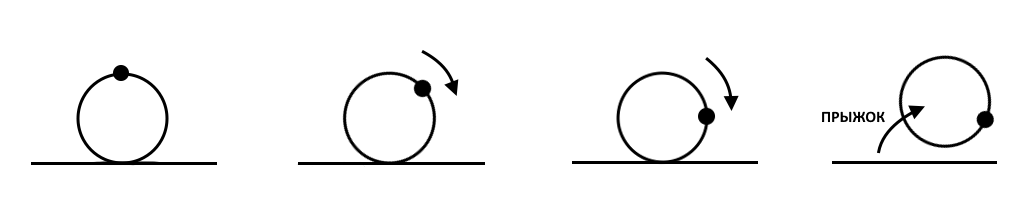
\includegraphics[width=1\textwidth]{hop-scheme.png}
	\caption{\textit{Процесс прыжка во время вращательного движения}}
	\label{hop-scheme}
\end{figure}

Когда колесо не подпрыгивает, точечная масса движется по циклоиде. Если бы в какой-то момент времени колесо пропало, то точечная масса двигалась бы по параболической траектории, причём такая траектория касательна к циклоиде. То есть при движении масса пытается двигаться по параболе, но она закреплена на диске. То есть данный эффект возникает, когда масса пытается двигаться по параболе и тянет за собой диск.

\begin{figure}[h!]
        \centering
	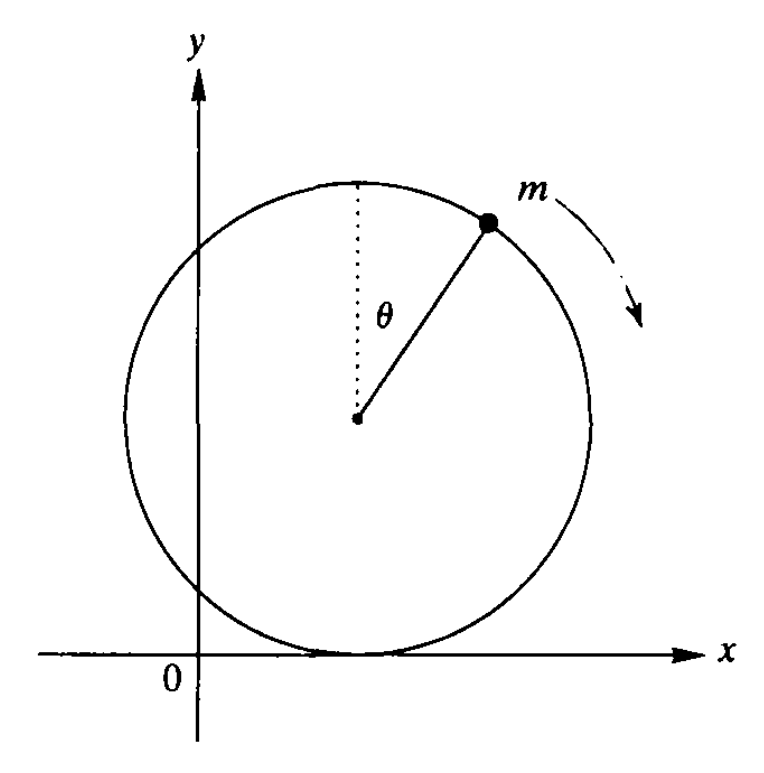
\includegraphics[width=0.6\textwidth]{roll-scheme.png}
	\caption{\textit{Колесо во время вращения}}
	\label{roll-scheme}
\end{figure}

Рассмотрим этот эффект подробнее на примере диска, с закреплённой с краю точечной массой (рис. \ref{center-scheme}). При исследовании его движения будем рассматривать центр масс.

\begin{figure}[h!]
        \centering
	\includegraphics[width=0.6\textwidth]{center-scheme.png}
	\caption{\textit{Колесо во время вращения}}
	\label{center-scheme}
\end{figure}

Расстояние от центра диска до центра масс можно вычислить как

\begin{equation}
    r = \frac{mR}{M + m}
\end{equation}

где $M$ -- масса диска, $m$ -- масса дополнительного груза, $R$ -- радиус диска. Дальнейшее движение будем рассматривать как движение невесомого диска радиусом $r$, с закреплённой точечной массой $m_0$ на расстоянии $r$ от центра диска.

Рассмотрим процесс вращения, направим оси так, как показано на рисунке \ref{roll-scheme}. Для точечной массы запишем закон сохранения энергии:

\begin{equation}
    \frac{m_0(\dot{x}^2 + \dot{y}^2)}{2} + m_0gy = \frac{m_0 v_{0}^2}{2} + 2r m_0g
\end{equation}

Когда колесо не подпрыгивает, точечная масса движется по циклоиде. Запишем движение в этом случае в координатах:

\begin{equation}
    x(t) = r \theta(t) + r \sin{\theta(t)}
\end{equation}


\begin{equation}
    y(t) = r + r \cos{\theta(t)}
\end{equation}

Подставив эти соотношения в выражение для закона сохранения энергии, имеем:

\begin{equation}
    \frac{m_0}{2} \left( \left( r \dot{\theta} + r \cos{\theta} \cdot \dot{\theta} \right)^2  + \left( -r \sin{\theta} \cdot \dot{\theta} \right)^2 \right) + m_0g(r + r \cos{\theta}) = \frac{m_0 v_0^2}{2} + 2m_0gr
\end{equation}

Отсюда получаем, что

\begin{equation}
    \dot{\theta}^2 = \frac{4gr \sin^2{\frac{\theta}{2}} + v_0^2}{4 r^2 \cos^2{\frac{\theta}{2}}}
\end{equation}

Тогда можем представить $\dot{y}$ и $\ddot{y}$ как

\begin{equation}
    \dot{y} = -r \sin{\theta} \cdot \dot{\theta} = - \sin{\frac{\theta}{2}} \sqrt{4gr \sin^2{\frac{\theta}{2}} + v_0^2}
\end{equation}

\begin{equation}
    \ddot{y} = -2g \sin^2{\frac{\theta}{2}} - \frac{v_0^2}{4r}
\end{equation}

Так как масса $m_0$ тянет диск вверх для прыжка и двигать его по параболе, поэтому прыжок произойдёт в тот момент, когда производная движения массы превысит производную циклоиды, то есть прыжок возникает при минимальном $\theta$ таком, что $-g \ge \ddot{y}(\theta(t))$, а если преобразовать, то

\begin{equation}\label{angle-speed}
    \sin{\frac{\theta}{2}} \ge \frac{1}{\sqrt{2}} \left( 1 - \frac{v_0^2}{4gr} \right)^{1/2}
\end{equation}

Так же можно получить выражение для минимальной начальной скорости, чтобы колесо подпрыгнуло при угле $\theta$:

\begin{equation}
    v_0 \ge \sqrt{4gr - 8gr \sin^2{\frac{\theta}{2}}}
\end{equation}

Отсюда следует, что при начальной скорости $v_0 \ge \sqrt{4gr}$ колесо подпрыгнет всегда в какой-то момент движения. Тогда подставим выражение для $r$:

\begin{equation}
    v_0 = \sqrt{4g \frac{mR}{M + m}}
\end{equation}

\section{Эксперимент}

Для эксперимента будем использовать два различных колеса, первое представляет собой картонный диск массой $M_1 = (22,7 \pm 0,1)$ г и радиусом $R_1 = (15,0 \pm 0,1)$ см, точечная масса для него $m_1 = (29,4 \pm 0,1)$ г. 

Второе колесо является крышкой (полым цилиндром, у которого отсутствует одна стенка) массой $M_2 = (12,3 \pm 0,1)$ г и радиусом $R_2 = (6,0 \pm 0,1)$ см, груз имеет массу $m_2 = (23,6 \pm 0,1)$ г.

Во время эксперимента будем закручивать колёса с различными начальными скоростями и наблюдать, будет ли колесо подпрыгивать. По видео оценим начальную скорость движения. Воспользуемся методом пропорций: зная параметры колёс можно оценить расстояние, пройденное телом, составив пропрцию. Время оценим по кадрам, пройденным за время движения.

Для показанного видео оценка скорости составляет $v_0 \approx 63,5 \text{см}/\text{с}$, а угол приблизительно 30 градусов, что соответствует теоретической оценке \ref{angle-speed}.

\section{Анализ данных и выводы}

Как показано на видео эксперимент прошёл удачно и эффект наблюдался. Экспериментальное значение скорости соответствует теоретическому. Отсюда можно судить, что теоритическая оценка верна.

\section{Список литературы}

\begin{itemize}
    \item Tokieda, T. F. (1997). The Hopping Hoop. The American Mathematical Monthly, 104(2), 152–154. doi:10.1080/00029890.1997.11990614 
    \item Willem F.D. Theron. Analysis of the Rolling Motion of Loaded Hoops
\end{itemize}

\end{document}
